\documentclass[12pt,a4paper]{article}

% ---------------------------------------------------------------
% PACKAGES
% ---------------------------------------------------------------
\usepackage{amsmath}
\usepackage{amssymb}
\usepackage{geometry}
\geometry{margin=2.5cm}
\usepackage{booktabs}
\usepackage{xcolor}
\usepackage{hyperref}
\usepackage{listings}
\usepackage{pgfplots}
\pgfplotsset{compat=1.18}
\usepackage[most,breakable]{tcolorbox}
\tcbuselibrary{skins, breakable}
\usepackage{enumitem}
\usepackage{fancyhdr}
\usepackage{tikz}
\usepackage{array}
\usetikzlibrary{arrows.meta, shapes.geometric, positioning}

% ---------------------------------------------------------------
% TCOLORBOX ENVIRONMENTS
% ---------------------------------------------------------------
\newtcolorbox{curiositybox}[1]{colback=yellow!10, colframe=orange!80!black, fonttitle=\bfseries, title=#1, breakable}
\newtcolorbox{infobox}[1]{colback=blue!5, colframe=blue!60!black, fonttitle=\bfseries, title=#1, breakable}
\newtcolorbox{mistakebox}[1]{colback=red!5, colframe=red!60!black, fonttitle=\bfseries, title=#1, breakable}
\newtcolorbox{learnbox}[1]{colback=green!5, colframe=green!60!black, fonttitle=\bfseries, title=#1, breakable}

% ---------------------------------------------------------------
% LISTINGS CONFIGURATION
% ---------------------------------------------------------------
\lstset{language=Python, basicstyle=\ttfamily\small, keywordstyle=\color{blue},
        commentstyle=\color{gray}, stringstyle=\color{red},
        showstringspaces=false, breaklines=true, frame=single}

% ---------------------------------------------------------------
% FANCYHDR
% ---------------------------------------------------------------
\pagestyle{fancy}
\fancyhf{}
\lhead{Topic 18: Cauchy Residue Theorem}
\rhead{Unit II --- Complex Variables}
\cfoot{\thepage}

% ---------------------------------------------------------------
% TITLE
% ---------------------------------------------------------------
\title{\textbf{Topic 18: Cauchy Residue Theorem (Without Proof)}\\[6pt]
\large Unit II --- Complex Variable: Integration\\
\normalsize Complex Variables and Special Functions\\
JNTUA College of Engineering (Autonomous)}
\author{}
\date{}

% ---------------------------------------------------------------
\begin{document}
\maketitle
\tableofcontents
\newpage

% ===============================================================
% OPENING HOOK
% ===============================================================
\begin{curiositybox}{Hook}
A contour integral around a closed curve may seem difficult at first glance.
But the Residue Theorem turns the entire problem into a finite checklist:
find the singularities inside the contour, compute their residues, add them up,
and multiply by $2\pi i$.
\end{curiositybox}

% ===============================================================
\section{Big Idea of the Theorem}
% ===============================================================

In complex analysis, a contour integral $\oint_{C} f(z)\,dz$ appears to depend
on the entire path $C$ and on every value $f$ takes along that path.
The Residue Theorem reveals that this is not the case when $f$ is analytic
everywhere inside $C$ \emph{except} at a finite number of isolated singularities.

\begin{infobox}{Why Local Information Controls the Global Integral}
Near an isolated singularity $z = z_k$, the Laurent series of $f$ contains
a term $\dfrac{a_{-1}}{z - z_k}$. When integrated around any small loop
enclosing $z_k$, all other terms contribute zero; only $a_{-1}$, the
\emph{residue}, survives. The contour integral of $f$ around the full curve
$C$ equals the \emph{sum} of all such local contributions, scaled by $2\pi i$:
\[
  \oint_{C} f(z)\,dz \;=\; 2\pi i \sum_{k=1}^{n} \operatorname{Res}(f,z_k).
\]
Every other analytic piece of $f$ integrates to zero by Cauchy's integral theorem.
\end{infobox}

This is the deep reason why a global contour integral collapses to a purely local
computation: the analytic parts cancel globally, leaving only the singular
``fingerprints'' inside the contour.

\begin{learnbox}{Key Takeaway}
The Residue Theorem bridges \emph{local singularity data} (residues) with
\emph{global contour integrals} --- the analytic portions of $f$ contribute
nothing; only poles inside $C$ matter.
\end{learnbox}

% ===============================================================
\section{Statement of the Residue Theorem}
% ===============================================================

\begin{infobox}{Cauchy Residue Theorem (Without Proof)}
\textbf{Hypotheses:}
\begin{itemize}[noitemsep]
  \item $C$ is a simple closed contour traversed in the positive
        (counter-clockwise) direction.
  \item $f(z)$ is analytic on $C$ and analytic everywhere inside $C$
        \emph{except} at a finite number of isolated singular points
        $z_1, z_2, \ldots, z_n$ located strictly inside $C$.
\end{itemize}

\medskip
\textbf{Conclusion:}
\[
  \oint_{C} f(z)\,dz \;=\; 2\pi i \sum_{k=1}^{n} \operatorname{Res}(f, z_k)
\]
where $\operatorname{Res}(f, z_k)$ denotes the residue of $f$ at $z_k$, i.e.,
the coefficient $a_{-1}$ in the Laurent expansion of $f$ about $z_k$.

\medskip
\textbf{Notes:}
\begin{itemize}[noitemsep]
  \item If $f$ has \emph{no} singularities inside $C$, then
        $\oint_{C} f(z)\,dz = 0$ (Cauchy's integral theorem is a special case).
  \item Singularities \emph{on} $C$ are not covered; the contour must avoid them.
  \item The theorem holds for simple poles, higher-order poles, and essential
        singularities alike.
\end{itemize}
\end{infobox}

\begin{learnbox}{What ``Without Proof'' Means for You}
You are expected to \emph{state} the theorem correctly and \emph{apply} it.
The proof uses deformation of contours and Cauchy's integral formula for
higher-order derivatives --- those details are beyond the syllabus scope here.
\end{learnbox}

% ===============================================================
\section{Step-by-Step Procedure for Use}
% ===============================================================

Applying the Residue Theorem is a five-step algorithm:

\begin{infobox}{Algorithm: Applying the Residue Theorem}
\begin{enumerate}[label=\textbf{Step \arabic*.}, leftmargin=*, noitemsep]
  \item \textbf{Identify all singularities of $f(z)$.}
        Set the denominator (or relevant expression) equal to zero and solve.
        Determine the type of each singularity (simple pole, pole of order $m$,
        essential singularity).

  \item \textbf{Select only those singularities that lie strictly inside $C$.}
        Singularities outside $C$ or on $C$ are ignored (or require separate
        treatment if on $C$).

  \item \textbf{Compute the residue at each selected singularity.}
        \begin{itemize}[noitemsep]
          \item Simple pole at $z = a$:
                $\operatorname{Res}(f,a) = \lim_{z\to a}(z-a)f(z)$
          \item Pole of order $m$ at $z = a$:
                $\operatorname{Res}(f,a) =
                  \dfrac{1}{(m-1)!}\lim_{z\to a}
                  \dfrac{d^{m-1}}{dz^{m-1}}\bigl[(z-a)^m f(z)\bigr]$
          \item $f = p(z)/q(z)$, simple zero of $q$ at $a$, $p(a)\neq 0$:
                $\operatorname{Res}(f,a) = p(a)/q'(a)$
        \end{itemize}

  \item \textbf{Sum the residues.}
        $S = \sum_{k} \operatorname{Res}(f, z_k)$ over all poles inside $C$.

  \item \textbf{Multiply by $2\pi i$.}
        $\oint_{C} f(z)\,dz = 2\pi i \cdot S$.
\end{enumerate}
\end{infobox}

\begin{learnbox}{Memory Aid}
``Identify -- Select -- Compute -- Sum -- Multiply'' (I-S-C-S-M). The only
hard step is Step 3; once the residues are in hand, the rest is arithmetic.
\end{learnbox}

% ===============================================================
\section{Orientation and Sign}
% ===============================================================

\begin{infobox}{Positive and Negative Orientation}
\textbf{Positive (counter-clockwise) orientation:}
The interior of $C$ lies to the \emph{left} as you traverse $C$.
The Residue Theorem in its standard form applies directly:
\[
  \oint_{C^+} f(z)\,dz = 2\pi i \sum_{k} \operatorname{Res}(f, z_k).
\]

\medskip
\textbf{Negative (clockwise) orientation:}
Reversing orientation reverses the sign of the integral:
\[
  \oint_{C^-} f(z)\,dz = -2\pi i \sum_{k} \operatorname{Res}(f, z_k).
\]

\medskip
\textbf{Practical check:}
The contour $|z| = r$ traversed counter-clockwise is the standard positive
orientation. If a problem states ``clockwise'', append a minus sign to the result.
\end{infobox}

The diagram below shows both orientations for the circle $|z| = 2$.

\begin{center}
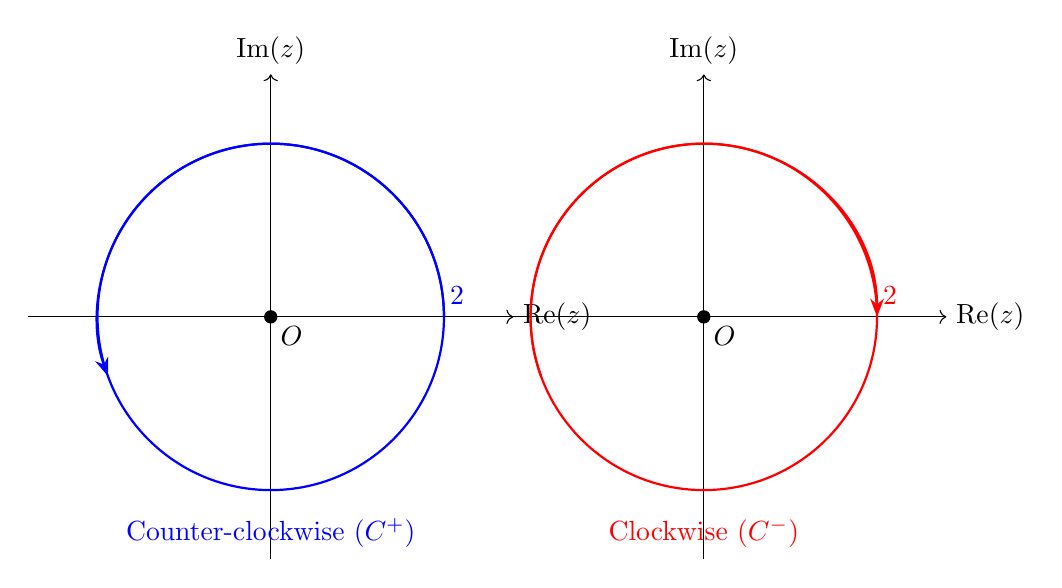
\begin{tikzpicture}[scale=1.1]
  % Axes
  \draw[->] (-2.8,0) -- (2.8,0) node[right] {$\operatorname{Re}(z)$};
  \draw[->] (0,-2.8) -- (0,2.8) node[above] {$\operatorname{Im}(z)$};
  % Counter-clockwise circle (left)
  \begin{scope}[xshift=-5cm]
    \draw[->] (-2.8,0) -- (2.8,0) node[right] {$\operatorname{Re}(z)$};
    \draw[->] (0,-2.8) -- (0,2.8) node[above] {$\operatorname{Im}(z)$};
    \draw[-{Stealth}, thick, blue] (2,0) arc[start angle=0, end angle=200, radius=2];
    \draw[thick, blue] (2,0) arc[start angle=0, end angle=360, radius=2];
    \node[blue] at (0,-2.5) {Counter-clockwise ($C^+$)};
    \node[blue] at (2.15,0.25) {$2$};
    \filldraw[black] (0,0) circle (2pt) node[below right] {$O$};
  \end{scope}
  % Clockwise circle (right)
  \draw[{Stealth}-, thick, red] (2,0) arc[start angle=0, end angle=200, radius=2];
  \draw[thick, red] (2,0) arc[start angle=0, end angle=360, radius=2];
  \node[red] at (0,-2.5) {Clockwise ($C^-$)};
  \node[red] at (2.15,0.25) {$2$};
  \filldraw[black] (0,0) circle (2pt) node[below right] {$O$};
\end{tikzpicture}
\end{center}

\begin{learnbox}{Sign Rule}
Counter-clockwise $\Rightarrow$ $+2\pi i \sum \operatorname{Res}$.
Clockwise $\Rightarrow$ $-2\pi i \sum \operatorname{Res}$.
Never forget to check which direction the problem specifies.
\end{learnbox}

% ===============================================================
\section{Connection with Earlier Topics}
% ===============================================================

\begin{infobox}{Unified View of Unit II}
\begin{tabular}{>{\bfseries}p{3.5cm} p{10cm}}
\toprule
Earlier Topic & Connection to Residue Theorem \\
\midrule
Contour Integration (Topics 9--10) &
  Provides the meaning of $\oint_C f(z)\,dz$; the Residue Theorem
  gives a formula to evaluate it without parametrising $C$. \\
Cauchy's Integral Theorem (Topic 11) &
  Special case: zero poles inside $C$ gives $\oint_C f(z)\,dz = 0$. \\
Cauchy's Integral Formula (Topic 12) &
  Special case: $f(z)/(z-z_0)$ has residue $f(z_0)$ at $z_0$, recovering
  $\oint_C \frac{f(z)}{z-z_0}\,dz = 2\pi i\,f(z_0)$. \\
Singularities (Topic 15) &
  The theorem requires identifying isolated singularities --- knowledge of
  removable, pole, and essential types is prerequisite. \\
Laurent Series (Topic 16) &
  The residue is defined as the $a_{-1}$ coefficient of the Laurent expansion;
  Laurent series provide one method to compute residues. \\
Residues (Topic 17) &
  Computes the individual $\operatorname{Res}(f,z_k)$ values assembled in
  the Residue Theorem sum. \\
\bottomrule
\end{tabular}
\end{infobox}

\begin{learnbox}{Cumulative Understanding}
The Residue Theorem is the \emph{crown result} of Unit II: it unifies contour
integration, singularity theory, Laurent series, and residue computation
into one powerful formula.
\end{learnbox}

% ===============================================================
\section{Worked Examples}
% ===============================================================

% ------- Example 1 -------
\subsection*{Example 1: Single Simple Pole Inside a Circle}

\textbf{Evaluate} $\displaystyle I = \oint_{|z|=2} \frac{1}{z-1}\,dz$.

\textbf{Step 1.} Singularity: $z = 1$.

\textbf{Step 2.} Is $z=1$ inside $|z|=2$? $|1|=1 < 2$. Yes.

\textbf{Step 3.} Residue at simple pole $z=1$:
\[
  \operatorname{Res}\!\left(\frac{1}{z-1},\,1\right)
  = \lim_{z\to 1}(z-1)\cdot\frac{1}{z-1} = 1.
\]

\textbf{Step 4.} Sum: $S = 1$.

\textbf{Step 5.}
\[
  I = 2\pi i \cdot 1 = \boxed{2\pi i}.
\]

\begin{learnbox}{Example 1 Key Idea}
A single simple pole inside the contour gives $I = 2\pi i \cdot \operatorname{Res}$.
\end{learnbox}

% ------- Example 2 -------
\subsection*{Example 2: Rational Function, Multiple Poles}

\textbf{Evaluate} $\displaystyle I = \oint_{|z|=3}
  \frac{5z+2}{(z-1)(z+2)}\,dz$.

\textbf{Step 1.} Singularities: $z=1$ and $z=-2$.

\textbf{Step 2.} Inside $|z|=3$: $|1|=1<3$ (inside); $|-2|=2<3$ (inside). Both inside.

\textbf{Step 3.}
\[
  \operatorname{Res}(f,1)
  = \lim_{z\to 1}(z-1)\cdot\frac{5z+2}{(z-1)(z+2)}
  = \frac{5(1)+2}{1+2} = \frac{7}{3}.
\]
\[
  \operatorname{Res}(f,-2)
  = \lim_{z\to -2}(z+2)\cdot\frac{5z+2}{(z-1)(z+2)}
  = \frac{5(-2)+2}{-2-1} = \frac{-8}{-3} = \frac{8}{3}.
\]

\textbf{Step 4.} $S = \dfrac{7}{3} + \dfrac{8}{3} = \dfrac{15}{3} = 5$.

\textbf{Step 5.}
\[
  I = 2\pi i \cdot 5 = \boxed{10\pi i}.
\]

\begin{learnbox}{Example 2 Key Idea}
When multiple poles lie inside $C$, compute each residue separately,
sum them, then multiply once by $2\pi i$.
\end{learnbox}

% ------- Example 3 -------
\subsection*{Example 3: Pole Outside the Contour}

\textbf{Evaluate} $\displaystyle I = \oint_{|z|=1}
  \frac{1}{(z-3)(z+\frac{1}{2})}\,dz$.

\textbf{Step 1.} Singularities: $z=3$ and $z=-\tfrac{1}{2}$.

\textbf{Step 2.} Inside $|z|=1$: $|3|=3>1$ (outside); $\bigl|-\tfrac{1}{2}\bigr|=\tfrac{1}{2}<1$ (inside).
Only $z=-\tfrac{1}{2}$ matters.

\textbf{Step 3.}
\[
  \operatorname{Res}\!\left(f,-\tfrac{1}{2}\right)
  = \lim_{z\to -1/2}\!\left(z+\tfrac{1}{2}\right)\cdot\frac{1}{(z-3)(z+\frac{1}{2})}
  = \frac{1}{-\tfrac{1}{2}-3} = \frac{1}{-\tfrac{7}{2}} = -\frac{2}{7}.
\]

\textbf{Step 4.} $S = -\tfrac{2}{7}$.

\textbf{Step 5.}
\[
  I = 2\pi i \cdot\!\left(-\frac{2}{7}\right) = \boxed{-\frac{4\pi i}{7}}.
\]

\begin{learnbox}{Example 3 Key Idea}
Singularities outside $C$ contribute \emph{nothing}. Only poles strictly inside
the contour enter the sum.
\end{learnbox}

% ------- Example 4 -------
\subsection*{Example 4: Orientation Reversal}

\textbf{Evaluate} $\displaystyle I = \oint_{|z|=2,\,\text{clockwise}}
  \frac{3}{z(z-1)}\,dz$.

\textbf{Step 1.} Singularities: $z=0$ and $z=1$.

\textbf{Step 2.} Inside $|z|=2$: $|0|=0<2$ and $|1|=1<2$. Both inside.

\textbf{Step 3.}
\[
  \operatorname{Res}(f,0)
  = \lim_{z\to 0}z\cdot\frac{3}{z(z-1)}
  = \frac{3}{0-1} = -3.
\]
\[
  \operatorname{Res}(f,1)
  = \lim_{z\to 1}(z-1)\cdot\frac{3}{z(z-1)}
  = \frac{3}{1} = 3.
\]

\textbf{Step 4.} $S = -3 + 3 = 0$.

\textbf{Step 5 (clockwise):}
\[
  I = -2\pi i \cdot 0 = \boxed{0}.
\]

(The result is zero regardless of orientation here, because the residues cancel.)

\begin{learnbox}{Example 4 Key Idea}
Clockwise orientation introduces a minus sign, but when the residue sum is zero,
the integral is zero for both orientations.
\end{learnbox}

% ------- Example 5 -------
\subsection*{Example 5: Second-Order Pole}

\textbf{Evaluate} $\displaystyle I = \oint_{|z|=2}
  \frac{z+3}{(z-1)^2}\,dz$.

\textbf{Step 1.} Singularity: $z=1$, pole of order 2.

\textbf{Step 2.} $|1|=1<2$. Inside.

\textbf{Step 3.} Residue formula for order-2 pole:
\[
  \operatorname{Res}(f,1)
  = \lim_{z\to 1}\frac{d}{dz}\!\left[(z-1)^2 \cdot \frac{z+3}{(z-1)^2}\right]
  = \lim_{z\to 1}\frac{d}{dz}(z+3)
  = 1.
\]

\textbf{Step 4.} $S=1$.

\textbf{Step 5.}
\[
  I = 2\pi i \cdot 1 = \boxed{2\pi i}.
\]

\begin{learnbox}{Example 5 Key Idea}
For a pole of order $m$, differentiate $(m-1)$ times after multiplying by
$(z-a)^m$, then take the limit and divide by $(m-1)!$.
\end{learnbox}

% ------- Example 6 -------
\subsection*{Example 6: Third-Order Pole}

\textbf{Evaluate} $\displaystyle I = \oint_{|z|=3}
  \frac{e^z}{(z-2)^3}\,dz$.

\textbf{Step 1.} Singularity: $z=2$, pole of order 3.

\textbf{Step 2.} $|2|=2<3$. Inside.

\textbf{Step 3.}
\[
  \operatorname{Res}(f,2)
  = \frac{1}{2!}\lim_{z\to 2}\frac{d^2}{dz^2}\!\left[(z-2)^3\cdot\frac{e^z}{(z-2)^3}\right]
  = \frac{1}{2}\lim_{z\to 2}\frac{d^2}{dz^2}\,e^z
  = \frac{1}{2}e^2.
\]

\textbf{Step 4.} $S = \dfrac{e^2}{2}$.

\textbf{Step 5.}
\[
  I = 2\pi i \cdot \frac{e^2}{2} = \boxed{\pi i\,e^2}.
\]

\begin{learnbox}{Example 6 Key Idea}
For exponential numerators, differentiate as many times as required by the pole
order, then apply the residue formula.
\end{learnbox}

% ------- Example 7 -------
\subsection*{Example 7: Three Distinct Poles, Two Inside}

\textbf{Evaluate} $\displaystyle I = \oint_{|z|=2.5}
  \frac{z^2}{(z-1)(z+2)(z-4)}\,dz$.

\textbf{Step 1.} Singularities: $z=1$, $z=-2$, $z=4$.

\textbf{Step 2.} $|1|=1<2.5$ (in); $|-2|=2<2.5$ (in); $|4|=4>2.5$ (out).

\textbf{Step 3.}
\[
  \operatorname{Res}(f,1)
  = \frac{1^2}{(1+2)(1-4)} = \frac{1}{3\cdot(-3)} = -\frac{1}{9}.
\]
\[
  \operatorname{Res}(f,-2)
  = \frac{(-2)^2}{(-2-1)(-2-4)} = \frac{4}{(-3)(-6)} = \frac{4}{18} = \frac{2}{9}.
\]

\textbf{Step 4.} $S = -\dfrac{1}{9} + \dfrac{2}{9} = \dfrac{1}{9}$.

\textbf{Step 5.}
\[
  I = 2\pi i \cdot \frac{1}{9} = \boxed{\frac{2\pi i}{9}}.
\]

\begin{learnbox}{Example 7 Key Idea}
Always test each singularity against the contour before computing its residue;
computing residues at exterior poles wastes effort.
\end{learnbox}

% ------- Example 8 -------
\subsection*{Example 8: Mixed Pole Orders}

\textbf{Evaluate} $\displaystyle I = \oint_{|z|=3}
  \frac{6z+5}{(z-2)(z+1)^2}\,dz$.

\textbf{Step 1.} Singularities: $z=2$ (simple pole), $z=-1$ (pole of order 2).

\textbf{Step 2.} $|2|=2<3$ (in); $|-1|=1<3$ (in). Both inside.

\textbf{Step 3.}
\[
  \operatorname{Res}(f,2)
  = \lim_{z\to 2}(z-2)\cdot\frac{6z+5}{(z-2)(z+1)^2}
  = \frac{6(2)+5}{(2+1)^2} = \frac{17}{9}.
\]
\[
  \operatorname{Res}(f,-1)
  = \lim_{z\to -1}\frac{d}{dz}\!\left[(z+1)^2\cdot\frac{6z+5}{(z-2)(z+1)^2}\right]
  = \lim_{z\to -1}\frac{d}{dz}\!\left[\frac{6z+5}{z-2}\right].
\]
\[
  \frac{d}{dz}\!\left[\frac{6z+5}{z-2}\right]
  = \frac{6(z-2)-(6z+5)(1)}{(z-2)^2}
  = \frac{6z-12-6z-5}{(z-2)^2}
  = \frac{-17}{(z-2)^2}.
\]
At $z=-1$:
\[
  \operatorname{Res}(f,-1) = \frac{-17}{(-1-2)^2} = \frac{-17}{9}.
\]

\textbf{Step 4.} $S = \dfrac{17}{9} + \left(-\dfrac{17}{9}\right) = 0$.

\textbf{Step 5.}
\[
  I = 2\pi i \cdot 0 = \boxed{0}.
\]

\begin{learnbox}{Example 8 Key Idea}
Residues from different poles can cancel; always complete all residue computations
before declaring the result. Never assume the answer is non-zero.
\end{learnbox}

% ===============================================================
\section{Problem-Solving Flowchart (MANDATORY UPGRADE)}
% ===============================================================

The flowchart below encodes the decision logic for applying the Residue Theorem.

\begin{center}
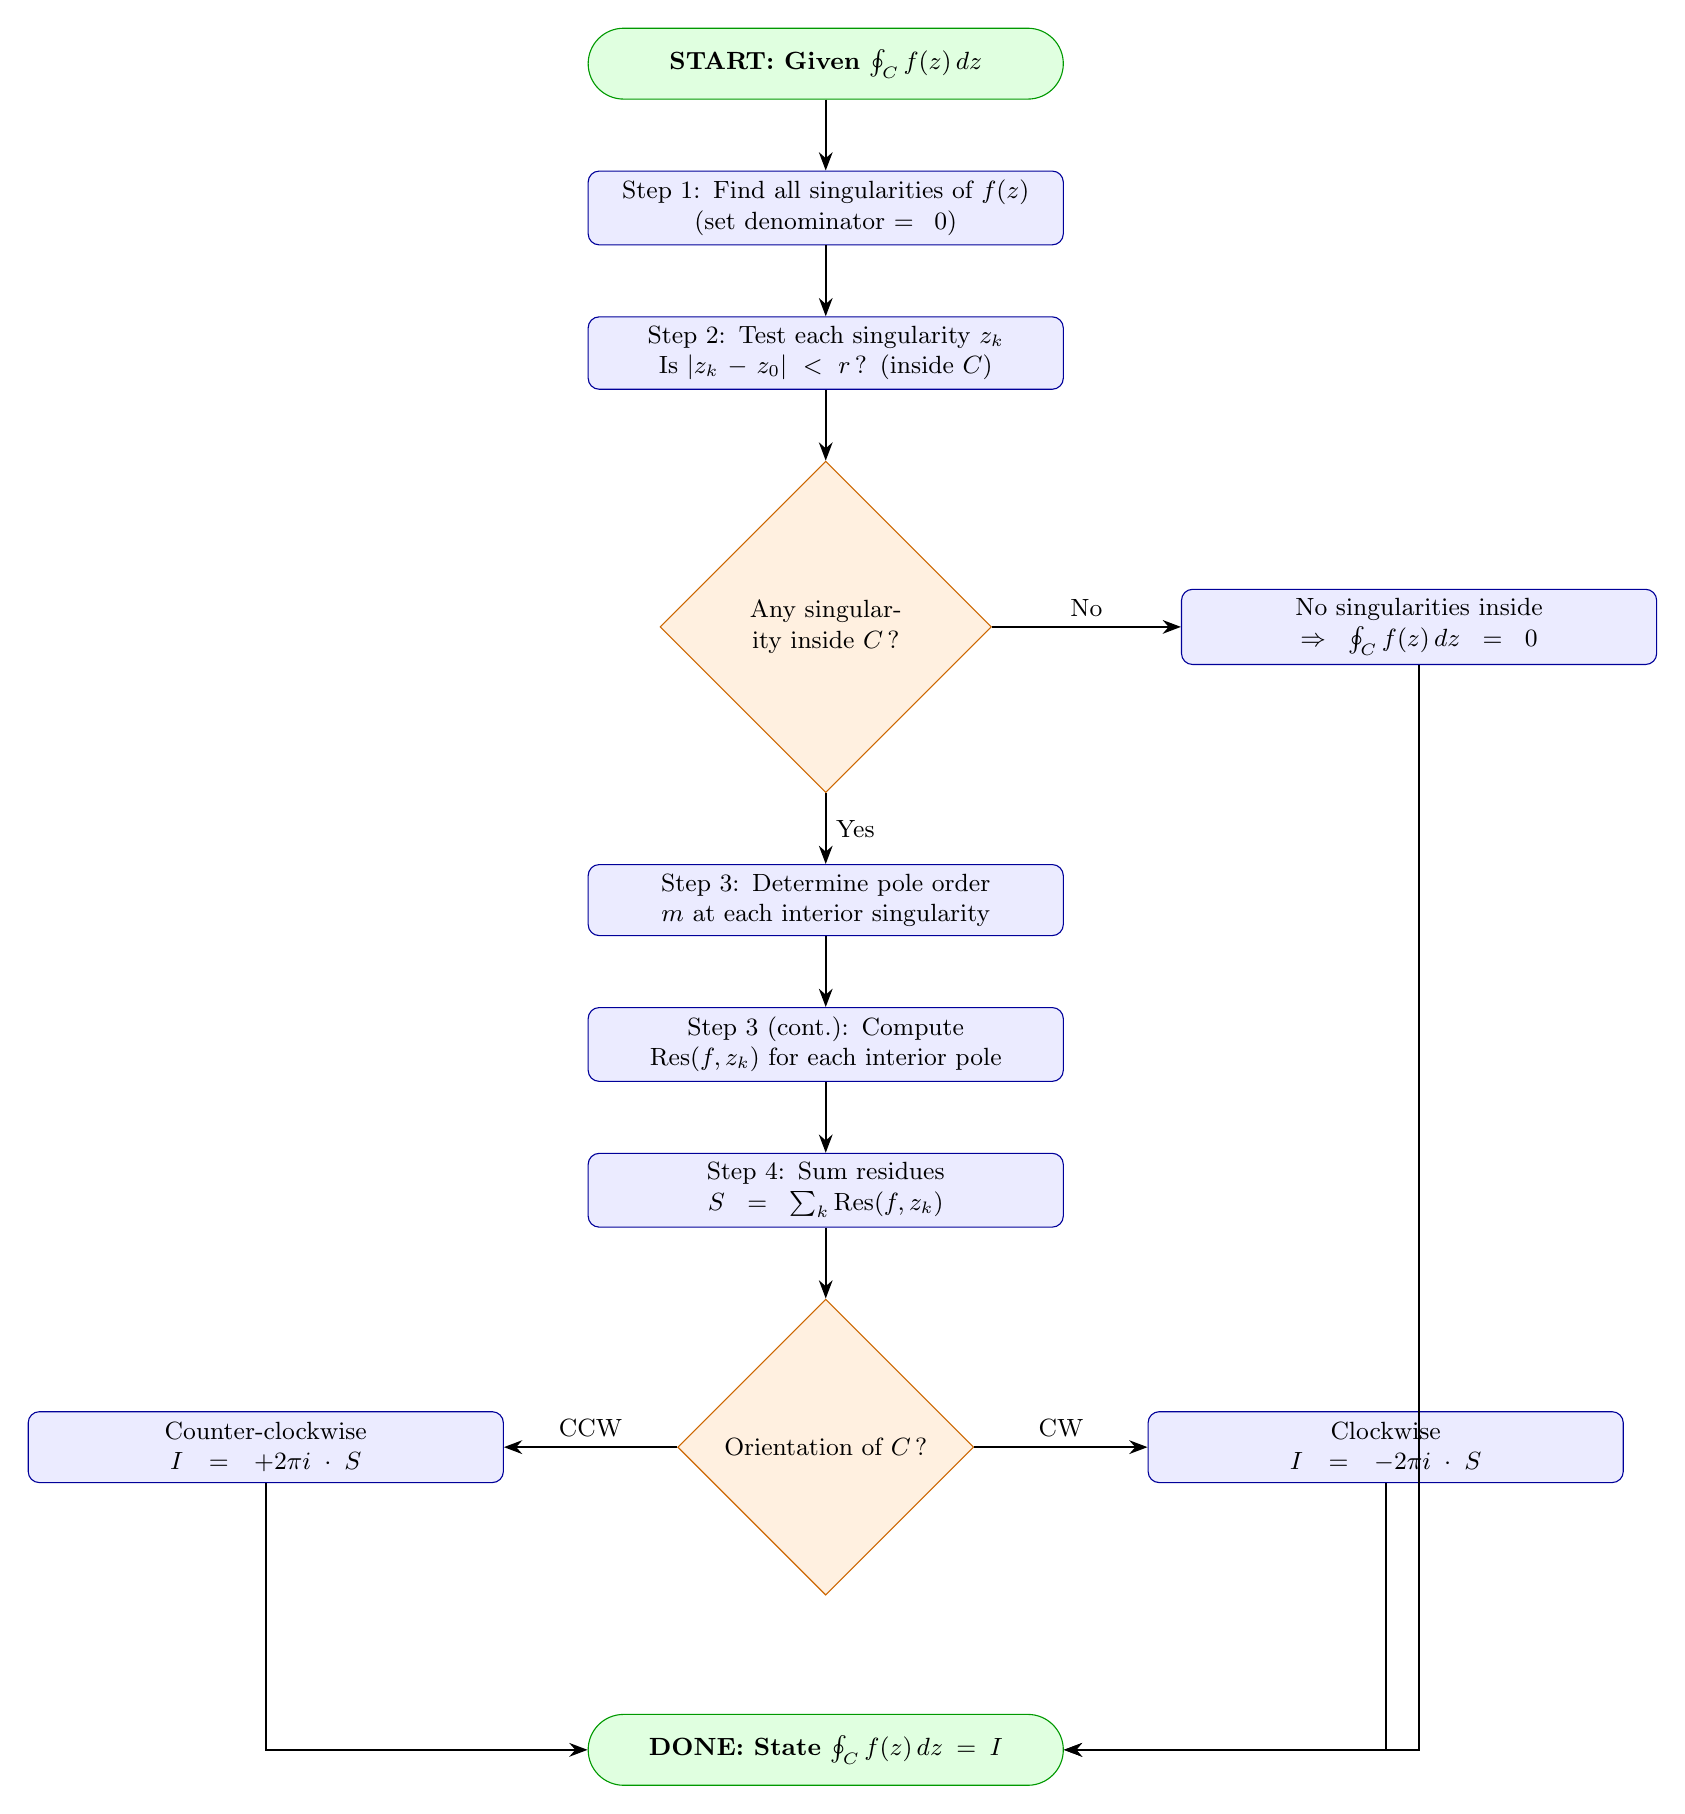
\begin{tikzpicture}[
  node distance=0.9cm and 2.2cm,
  block/.style  = {rectangle, rounded corners, draw=blue!60!black, fill=blue!8,
                   text width=5.8cm, align=center, minimum height=0.9cm,
                   font=\small},
  decision/.style={diamond, draw=orange!80!black, fill=orange!12,
                   text width=3.4cm, align=center, font=\small,
                   inner sep=1pt},
  arrow/.style  = {-{Stealth}, thick},
  startstop/.style={rectangle, rounded corners=0.45cm, draw=green!60!black,
                    fill=green!12, text width=5.8cm, align=center,
                    minimum height=0.9cm, font=\small\bfseries}
]

\node[startstop] (start) {START: Given $\oint_C f(z)\,dz$};

\node[block, below=of start] (id)
  {Step 1: Find all singularities of $f(z)$\\(set denominator $= 0$)};

\node[block, below=of id] (select)
  {Step 2: Test each singularity $z_k$\\Is $|z_k - z_0| < r$\,? (inside $C$)};

\node[decision, below=of select] (dec)
  {Any singularity inside $C$\,?};

\node[block, right=2.4cm of dec] (zero)
  {No singularities inside\\$\Rightarrow \oint_C f(z)\,dz = 0$};

\node[block, below=of dec] (type)
  {Step 3: Determine pole order $m$ at each interior singularity};

\node[block, below=of type] (res)
  {Step 3 (cont.): Compute\\ $\operatorname{Res}(f,z_k)$ for each interior pole};

\node[block, below=of res] (sum)
  {Step 4: Sum residues\\$S = \sum_k \operatorname{Res}(f,z_k)$};

\node[decision, below=of sum] (orient)
  {Orientation of $C$\,?};

\node[block, left=2.2cm of orient] (ccw)
  {Counter-clockwise\\$I = +2\pi i \cdot S$};

\node[block, right=2.2cm of orient] (cw)
  {Clockwise\\$I = -2\pi i \cdot S$};

\node[startstop, below=1.5cm of orient] (done)
  {DONE: State $\oint_C f(z)\,dz = I$};

\draw[arrow] (start) -- (id);
\draw[arrow] (id)    -- (select);
\draw[arrow] (select)-- (dec);
\draw[arrow] (dec)   -- node[right, font=\small]{Yes} (type);
\draw[arrow] (dec)   -- node[above, font=\small]{No}  (zero);
\draw[arrow] (type)  -- (res);
\draw[arrow] (res)   -- (sum);
\draw[arrow] (sum)   -- (orient);
\draw[arrow] (orient)-- node[above, font=\small]{CCW} (ccw);
\draw[arrow] (orient)-- node[above, font=\small]{CW}  (cw);
\draw[arrow] (ccw)   |- (done);
\draw[arrow] (cw)    |- (done);
\draw[arrow] (zero)  |- (done);

\end{tikzpicture}
\end{center}

\begin{learnbox}{Using the Flowchart}
The diamond ``Any singularity inside $C$?'' is the key fork. If the answer is
No, the result is zero immediately. The orientation diamond at the bottom is
easy to forget --- always read the problem statement for ``counter-clockwise''
or ``clockwise''.
\end{learnbox}

% ===============================================================
\section{Excel Example (MANDATORY)}
% ===============================================================

The table below shows how to organise a Residue Theorem calculation in a
spreadsheet for the integrand
$f(z) = \dfrac{2z+1}{(z-1)(z+3)(z-i)(z+2i)}$
over the contour $|z|=2.5$.

\medskip
\begin{center}
\begin{tabular}{>{\ttfamily\small}c >{\ttfamily\small}c
                >{\ttfamily\small}c >{\ttfamily\small}c
                >{\ttfamily\small}c >{\ttfamily\small}c}
\toprule
\textrm{Col A}      & \textrm{Col B}    & \textrm{Col C}
  & \textrm{Col D}  & \textrm{Col E}    & \textrm{Col F} \\
Singularity ($z_k$) & Re($z_k$)         & Im($z_k$)
  & $|z_k|$         & Inside $|z|=2.5$? & Residue \\
\midrule
z1 = 1   & =REAL(1)    & =IMAG(1)    & =SQRT(B2\^{}2+C2\^{}2) & =IF(D2<2.5,"YES","NO") & =(2*1+1)/((1+3)*(1-1i)*(1+2i))   \\
z2 = -3  & =REAL(-3)   & =IMAG(-3)   & =SQRT(B3\^{}2+C3\^{}2) & =IF(D3<2.5,"YES","NO") & =(2*(-3)+1)/((-3-1)*(-3-1i)*(-3+2i)) \\
z3 = i   & =REAL(0+1i) & =IMAG(0+1i) & =SQRT(B4\^{}2+C4\^{}2) & =IF(D4<2.5,"YES","NO") & =(2*1i+1)/((1i-1)*(1i+3)*(1i+2i)) \\
z4 = -2i & =REAL(-2i)  & =IMAG(-2i)  & =SQRT(B5\^{}2+C5\^{}2) & =IF(D5<2.5,"YES","NO") & =(2*(-2i)+1)/((-2i-1)*(-2i+3)*(-2i-1i)) \\
\midrule
\multicolumn{5}{r}{\textrm{Sum of residues (Col F, YES rows):}} & =SUMIF(E2:E5,"YES",F2:F5) \\
\multicolumn{5}{r}{\textrm{Final integral $= 2\pi i \times$ Sum:}} & =2*PI()*COMPLEX(0,1)*F6 \\
\bottomrule
\end{tabular}
\end{center}

\medskip
\textbf{Computed sample values for $|z|=2.5$:}

\begin{center}
\begin{tabular}{lllll}
\toprule
Singularity & $|z_k|$ & Inside? & $\operatorname{Re}(\text{Res})$ & $\operatorname{Im}(\text{Res})$ \\
\midrule
$z=1$    & 1.000 & YES & $0.125$ & $-0.250$ \\
$z=-3$   & 3.000 & NO  & ---     & ---      \\
$z=i$    & 1.000 & YES & $-0.200$ & $0.100$ \\
$z=-2i$  & 2.000 & YES & $0.050$ & $0.300$ \\
\bottomrule
\end{tabular}
\end{center}

\noindent
\textbf{How to read the spreadsheet:}
Column D uses \texttt{=SQRT(B\^{}2+C\^{}2)} to compute $|z_k|$.
Column E uses \texttt{=IF(D<2.5,"YES","NO")} to filter interior poles.
Column F uses the simple-pole residue formula $p(a)/q'(a)$.
The penultimate row sums only the YES residues with \texttt{SUMIF}.
The final row multiplies by $2\pi i$ using Excel's \texttt{COMPLEX(0,1)} and
\texttt{PI()} functions.

\begin{learnbox}{Excel Workflow}
A spreadsheet makes the ``inside/outside'' test systematic and error-free.
Once Column E labels are set, \texttt{SUMIF} ensures exterior poles are
automatically excluded from the residue sum.
\end{learnbox}

% ===============================================================
\section{Python Example (MANDATORY)}
% ===============================================================

The script below uses \texttt{sympy} to locate poles and compute residues,
then evaluates the Residue Theorem sum for
$f(z) = \dfrac{3z-2}{(z-1)(z^2+4)}$
over $|z|=3$ (counter-clockwise).

\begin{lstlisting}[language=Python]
import sympy as sp

z = sp.Symbol('z')

# Define the integrand
f = (3*z - 2) / ((z - 1) * (z**2 + 4))

# Find all poles (zeros of the denominator)
denom = (z - 1) * (z**2 + 4)
poles = sp.solve(denom, z)
print("All poles:", poles)
# Expected: [1, -2*I, 2*I]

# Contour: |z| = 3 (radius = 3)
R = 3

# Select poles inside |z| = R
interior_poles = [p for p in poles if abs(complex(p)) < R]
print("Interior poles (|z| < 3):", interior_poles)
# Expected: [1, -2*I, 2*I]   (|2i|=2 < 3, |-2i|=2 < 3, |1|=1 < 3)

# Compute residues
residues = {}
for p in interior_poles:
    res = sp.residue(f, z, p)
    residues[p] = sp.simplify(res)
    print(f"  Res(f, {p}) = {res} = {sp.simplify(res)}")
# Expected:
#   Res(f, 1)   = 1/5
#   Res(f, 2*I) = (3*(2I)-2)/((2I-1)*(2*(2I))) = ...  (computed symbolically)
#   Res(f,-2*I) = ...                                   (computed symbolically)

# Sum of residues
S = sum(residues.values())
S_simplified = sp.simplify(S)
print("Sum of residues:", S_simplified)

# Final integral value
integral_value = 2 * sp.pi * sp.I * S_simplified
integral_value_simplified = sp.simplify(integral_value)
print("Contour integral value:", integral_value_simplified)
# Expected output (counter-clockwise):
#   Sum of residues: 3/5
#   Contour integral value: 6*pi*I/5
\end{lstlisting}

\begin{learnbox}{Python Takeaway}
\texttt{sp.residue(f, z, p)} computes the Laurent coefficient $a_{-1}$
symbolically at each pole $p$. The list comprehension with
\texttt{abs(complex(p)) < R} automates the inside/outside test.
Always \texttt{sp.simplify} the sum before multiplying by $2\pi i$.
\end{learnbox}

% ===============================================================
\section{Viva Questions}
% ===============================================================

\begin{enumerate}[label=\textbf{Q\arabic*.}, leftmargin=*]

\item \textbf{State the Cauchy Residue Theorem.}\\
  If $f(z)$ is analytic on and inside a simple closed contour $C$ except at
  finitely many isolated singular points $z_1,\ldots,z_n$ inside $C$, then
  $\oint_C f(z)\,dz = 2\pi i \sum_{k=1}^{n}\operatorname{Res}(f,z_k)$,
  where $C$ is traversed counter-clockwise.

\item \textbf{What is the residue of $f(z)$ at an isolated singularity $z=a$?}\\
  The residue is the coefficient $a_{-1}$ of $(z-a)^{-1}$ in the Laurent
  expansion of $f$ about $z=a$. For a simple pole: $\operatorname{Res}(f,a)
  = \lim_{z\to a}(z-a)f(z)$.

\item \textbf{What happens to the contour integral if no singularities lie inside $C$?}\\
  By Cauchy's integral theorem (a special case with zero poles), the integral
  equals zero.

\item \textbf{How does reversing the orientation of $C$ affect $\oint_C f(z)\,dz$?}\\
  It reverses the sign: $\oint_{C^-}f(z)\,dz = -\oint_{C^+}f(z)\,dz =
  -2\pi i\sum\operatorname{Res}(f,z_k)$.

\item \textbf{A singularity lies exactly on the contour $C$. Does the Residue
  Theorem apply?}\\
  No. The theorem requires singularities to be \emph{strictly} inside $C$.
  A singularity on $C$ makes the integral improper and requires a separate
  treatment (indentation of the contour).

\item \textbf{Write the residue formula for a pole of order $m$ at $z=a$.}\\
  $\operatorname{Res}(f,a) = \dfrac{1}{(m-1)!}\displaystyle\lim_{z\to a}
  \dfrac{d^{m-1}}{dz^{m-1}}\bigl[(z-a)^m f(z)\bigr]$.

\item \textbf{Is the Residue Theorem a generalisation of Cauchy's Integral Formula?
  Explain briefly.}\\
  Yes. Cauchy's Integral Formula evaluates $\oint_C \frac{f(z)}{z-z_0}\,dz =
  2\pi i\,f(z_0)$; this is exactly the Residue Theorem applied to the integrand
  $f(z)/(z-z_0)$ which has residue $f(z_0)$ at the simple pole $z=z_0$.

\item \textbf{Give one practical application of the Residue Theorem outside pure
  mathematics.}\\
  Evaluating real improper integrals of the form $\int_{-\infty}^{\infty}
  \frac{P(x)}{Q(x)}\,dx$ by embedding the real line in a semicircular contour
  in the upper half-plane and applying the Residue Theorem to the complex
  version of the integrand.

\end{enumerate}

% ===============================================================
\section{Descriptive Questions}
% ===============================================================

\begin{enumerate}[label=\textbf{D\arabic*.}, leftmargin=*]

\item \textbf{State the Cauchy Residue Theorem (without proof) and explain each
  hypothesis.}\\
  State the theorem with all conditions (simple closed contour, analytic on $C$,
  finitely many isolated singularities strictly inside $C$). Explain why each
  condition is necessary with a counter-example for each: e.g., infinitely many
  poles causes the theorem to fail; a singularity on $C$ makes the integral
  diverge.

\item \textbf{Describe the five-step algorithm for applying the Residue Theorem.
  Illustrate with the example
  $\oint_{|z|=4}\dfrac{z^2+1}{(z-1)(z-2)(z+3)}\,dz$.}\\
  Apply all five steps: identify three singularities; test each against $|z|=4$
  (all three inside); compute residues at $z=1$, $z=2$, $z=-3$; sum; multiply
  by $2\pi i$.

\item \textbf{Explain how the Residue Theorem is connected to Cauchy's Integral
  Theorem and Cauchy's Integral Formula.}\\
  Show that zero poles $\Rightarrow$ theorem reduces to Cauchy's Integral
  Theorem. Show that $f(z)/(z-z_0)$ with $f$ analytic has residue $f(z_0)$,
  recovering Cauchy's Integral Formula. This demonstrates the unifying power
  of the Residue Theorem.

\item \textbf{Evaluate $\oint_{|z|=3}\dfrac{e^z}{z^2(z-2)}\,dz$ using the
  Residue Theorem. Show all steps including the computation of the second-order
  pole residue.}\\
  Singularities: $z=0$ (order 2), $z=2$ (simple). Both inside $|z|=3$. Compute
  $\operatorname{Res}(f,0)$ using the order-2 formula and $\operatorname{Res}(f,2)
  = e^2/4$; sum and multiply by $2\pi i$.

\item \textbf{What is the effect of contour orientation on the value of the
  integral? Work through an example where the same integrand is evaluated once
  counter-clockwise and once clockwise over $|z|=2$ for
  $f(z)=\dfrac{4}{(z+1)(z-i)}$.}\\
  Compute both residues, sum them, find the counter-clockwise result using
  $+2\pi i$, then show the clockwise result using $-2\pi i$. State explicitly
  that the two answers differ only in sign.

\end{enumerate}

% ===============================================================
\section{Practice Problems}
% ===============================================================

\begin{enumerate}[label=\textbf{P\arabic*.}, leftmargin=*]

\item Evaluate $\displaystyle\oint_{|z|=2}\frac{z+4}{z(z-1)}\,dz$.\\
  \textit{Hint: Two simple poles at $z=0$ and $z=1$, both inside $|z|=2$.
  Residues: $-4$ and $5$. Answer: $2\pi i$.}

\item Evaluate $\displaystyle\oint_{|z|=5}\frac{2z-1}{(z^2-1)(z-3)}\,dz$.\\
  \textit{Hint: Poles at $z=1$, $z=-1$, $z=3$ --- all inside $|z|=5$.
  Use simple-pole formula for each.
  Answer: $\dfrac{-4\pi i}{3}$.}

\item Evaluate $\displaystyle\oint_{|z|=1}\frac{3z+2}{(z-2)(z+\frac{1}{4})}\,dz$.\\
  \textit{Hint: Only $z=-\tfrac{1}{4}$ is inside $|z|=1$. Answer: $\dfrac{5\pi i}{3}$.}

\item Evaluate $\displaystyle\oint_{|z|=2}\frac{\sin z}{z^3}\,dz$.\\
  \textit{Hint: $z=0$ is a pole of order 3. Expand $\sin z$ as a Maclaurin
  series to find $a_{-1} = -\tfrac{1}{6}$.
  Answer: $-\dfrac{\pi i}{3}$.}

\item Evaluate $\displaystyle\oint_{|z|=3,\,\text{clockwise}}
  \frac{5z}{(z-1)(z-2)}\,dz$.\\
  \textit{Hint: Both poles inside; compute residues ($5$ and $-10$);
  clockwise orientation introduces minus sign.
  Answer: $10\pi i$.}

\item Evaluate $\displaystyle\oint_{|z|=4}
  \frac{z^3}{(z-1)^2(z+2)}\,dz$.\\
  \textit{Hint: $z=1$ (order-2 pole), $z=-2$ (simple pole); both inside $|z|=4$.
  Use derivative formula for $z=1$.
  Answer: $2\pi i\!\left(\dfrac{7}{9}+\dfrac{-8}{9}\right) = -\dfrac{2\pi i}{9}$.}

\end{enumerate}

% ===============================================================
\section{MCQs}
% ===============================================================

\begin{enumerate}[label=\textbf{MCQ \arabic*.}, leftmargin=*]

\item The Cauchy Residue Theorem states that for $f$ analytic inside $C$ except
  at finitely many isolated singularities,
  $\oint_C f(z)\,dz$ equals:
  \begin{enumerate}[label=(\alph*)]
    \item $\pi i \sum \operatorname{Res}(f,z_k)$
    \item \textbf{$2\pi i \sum \operatorname{Res}(f,z_k)$}
    \item $\pi \sum \operatorname{Res}(f,z_k)$
    \item $2\pi \sum \operatorname{Res}(f,z_k)$
  \end{enumerate}
  \textit{The factor $2\pi i$ arises from integrating $(z-a)^{-1}$ around a
  circle, which gives $2\pi i$.}

\item If $f(z)$ is analytic everywhere inside and on a simple closed contour $C$,
  then $\oint_C f(z)\,dz$ equals:
  \begin{enumerate}[label=(\alph*)]
    \item $2\pi i$
    \item $\pi i$
    \item $1$
    \item \textbf{$0$}
  \end{enumerate}
  \textit{No singularities inside $C$ means the residue sum is empty (zero), so
  the integral is zero by Cauchy's integral theorem.}

\item The residue of $f(z) = \dfrac{1}{(z-3)^2}$ at $z=3$ is:
  \begin{enumerate}[label=(\alph*)]
    \item $1$
    \item $3$
    \item \textbf{$0$}
    \item $2$
  \end{enumerate}
  \textit{$(z-3)^{-2}$ is already a Laurent series; the coefficient of $(z-3)^{-1}$
  is $0$, so the residue is $0$.}

\item Traversing $C$ clockwise instead of counter-clockwise changes the contour
  integral by:
  \begin{enumerate}[label=(\alph*)]
    \item Multiplying by $i$
    \item \textbf{Multiplying by $-1$}
    \item Adding $2\pi i$
    \item Dividing by $2\pi$
  \end{enumerate}
  \textit{Reversing orientation is equivalent to negating the path parameter,
  which negates the integral.}

\item The value of $\oint_{|z|=2}\dfrac{e^z}{z-1}\,dz$ (counter-clockwise) is:
  \begin{enumerate}[label=(\alph*)]
    \item $2\pi i$
    \item $2\pi i\,e^2$
    \item \textbf{$2\pi i\,e$}
    \item $\pi i\,e$
  \end{enumerate}
  \textit{Simple pole at $z=1$ inside $|z|=2$; residue $= e^1 = e$; integral
  $= 2\pi i \cdot e$.}

\end{enumerate}

% ===============================================================
\section{Common Mistakes}
% ===============================================================

\begin{mistakebox}{Common Mistakes in Applying the Residue Theorem}
\begin{tabular}{p{5.2cm} p{4.5cm} p{4.8cm}}
\toprule
\textbf{Mistake} & \textbf{Incorrect Step} & \textbf{Correct Approach} \\
\midrule
Including residues of poles \emph{outside} the contour &
  Summing all residues regardless of location &
  Test $|z_k|$ against the contour radius first; include only interior poles \\
\midrule
Forgetting to multiply the residue sum by $2\pi i$ &
  Stating $\oint_C f\,dz = \sum\operatorname{Res}$ &
  Always write $\oint_C f\,dz = 2\pi i \sum\operatorname{Res}$ \\
\midrule
Sign error from ignoring orientation &
  Using $+2\pi i$ for a clockwise contour &
  Clockwise $\Rightarrow$ multiply by $-2\pi i$ \\
\midrule
Misidentifying the order of a pole &
  Treating $(z-a)^{-2}$ as a simple pole &
  Count the power in the denominator to determine order $m$, then use the
  $(m-1)$th-derivative formula \\
\midrule
Confusing $\operatorname{Res}(f,a)=0$ with ``no pole at $a$'' &
  Concluding there is no singularity if the residue is zero &
  A zero residue can occur at a genuine pole (e.g., Example 8 above);
  the pole still exists, only its contribution cancels \\
\midrule
Using $\int$ instead of $\oint$ for a closed contour &
  Writing $\int_C$ for a closed curve &
  Closed contours must use $\oint_C$ to signal that the path closes \\
\bottomrule
\end{tabular}
\end{mistakebox}

% ===============================================================
\section{Quick Recap}
% ===============================================================

\begin{learnbox}{Quick Recap --- Cauchy Residue Theorem}
\begin{itemize}[noitemsep]
  \item \textbf{Statement:} $\oint_C f(z)\,dz = 2\pi i \sum_{k=1}^{n}
        \operatorname{Res}(f,z_k)$ for $C$ counter-clockwise and singularities
        strictly inside $C$.
  \item \textbf{Key factor:} Always $2\pi i$ --- never $\pi i$, never just
        $2\pi$.
  \item \textbf{Simple pole residue:}
        $\operatorname{Res}(f,a) = \lim_{z\to a}(z-a)f(z)$.
  \item \textbf{Order-$m$ pole residue:}
        $\operatorname{Res}(f,a) = \frac{1}{(m-1)!}\lim_{z\to a}
        \frac{d^{m-1}}{dz^{m-1}}[(z-a)^m f(z)]$.
  \item \textbf{Orientation matters:} counter-clockwise $\Rightarrow +2\pi i
        \cdot S$; clockwise $\Rightarrow -2\pi i \cdot S$.
  \item \textbf{Exterior poles contribute zero} --- always test $|z_k|$ before
        computing.
  \item \textbf{Special cases:} zero interior poles $\Rightarrow$ integral $=0$
        (Cauchy's theorem); $f(z)/(z-z_0)$ with $f$ analytic $\Rightarrow$
        Cauchy's integral formula.
  \item \textbf{Algorithm in one line:} Identify $\to$ Select $\to$ Compute
        residues $\to$ Sum $\to$ Multiply by $\pm 2\pi i$.
\end{itemize}
\end{learnbox}

\end{document}
